\begin{figure}[bth!]
	\begin{center}
		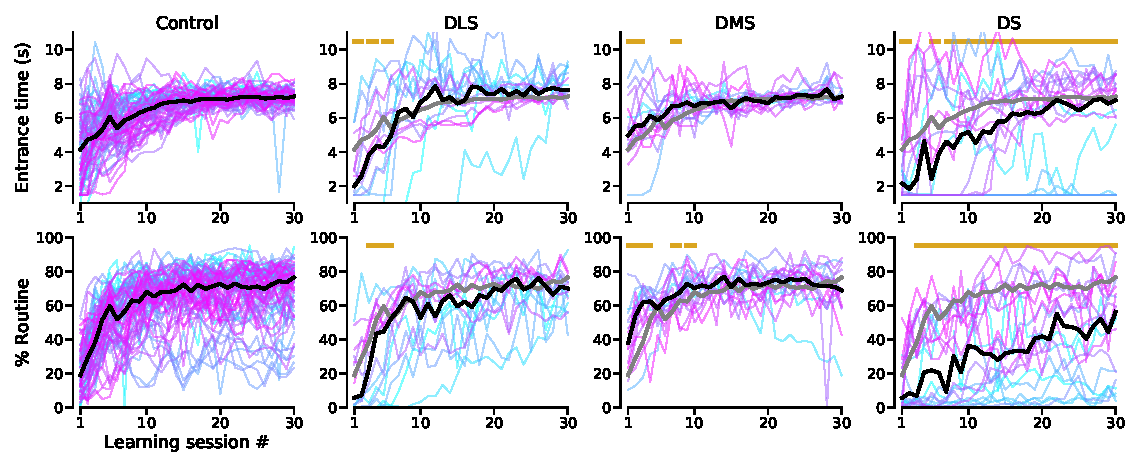
\includegraphics[width=\textwidth]{ch-lesion/figures/EarlyLesionLearning.pdf}
	   \caption
	   {\textbf{Effect of DLS, DMS and DS lesions performed before training on task learning.}
	   \textbf{(A)} Session-by-session change in performance ($ET$, upper panels; Percentage of trials in which the routine was used, lower panels) for animals without lesion (Control, left) and for animals that received a lesion before training (DLS, DMS, DS from left to right).
	   Black lines indicate Control group median.
	   Thin colored lines indicate single animals.
	   Thick colored lines (same color code as in Fig.~1) in 3 rightmost columns indicate group performance for comparison (8 lesion animals with fewer than 30 training sessions are not shown, which explains the difference in the number of animals in this figure and fig. S2C).
	   Horizontal golden lines indicate significant differences between control and lesion groups (corrected for multiple comparisons).
	   \textbf{(B)} Trajectories before and after extensive training (sessions \#1 and \#30) for two animals with large DS lesions. Note that, after extensive practice, R238 was capable of performing the wait-and-run routine.
	   \textbf{(C)} Percentage of trials in which animals remained in the front region of the treadmill (computed for sessions \#25 to \#30) versus lesion size.
	   }
	   \label{fig:lesion:EarlyLesionLearning}
	\end{center}
   \end{figure}